% Options for packages loaded elsewhere
\PassOptionsToPackage{unicode}{hyperref}
\PassOptionsToPackage{hyphens}{url}
%
\documentclass[
]{article}
\usepackage{amsmath,amssymb}
\usepackage{iftex}
\ifPDFTeX
  \usepackage[T1]{fontenc}
  \usepackage[utf8]{inputenc}
  \usepackage{textcomp} % provide euro and other symbols
\else % if luatex or xetex
  \usepackage{unicode-math} % this also loads fontspec
  \defaultfontfeatures{Scale=MatchLowercase}
  \defaultfontfeatures[\rmfamily]{Ligatures=TeX,Scale=1}
\fi
\usepackage{lmodern}
\ifPDFTeX\else
  % xetex/luatex font selection
\fi
% Use upquote if available, for straight quotes in verbatim environments
\IfFileExists{upquote.sty}{\usepackage{upquote}}{}
\IfFileExists{microtype.sty}{% use microtype if available
  \usepackage[]{microtype}
  \UseMicrotypeSet[protrusion]{basicmath} % disable protrusion for tt fonts
}{}
\makeatletter
\@ifundefined{KOMAClassName}{% if non-KOMA class
  \IfFileExists{parskip.sty}{%
    \usepackage{parskip}
  }{% else
    \setlength{\parindent}{0pt}
    \setlength{\parskip}{6pt plus 2pt minus 1pt}}
}{% if KOMA class
  \KOMAoptions{parskip=half}}
\makeatother
\usepackage{xcolor}
\usepackage[margin=1in]{geometry}
\usepackage{graphicx}
\makeatletter
\def\maxwidth{\ifdim\Gin@nat@width>\linewidth\linewidth\else\Gin@nat@width\fi}
\def\maxheight{\ifdim\Gin@nat@height>\textheight\textheight\else\Gin@nat@height\fi}
\makeatother
% Scale images if necessary, so that they will not overflow the page
% margins by default, and it is still possible to overwrite the defaults
% using explicit options in \includegraphics[width, height, ...]{}
\setkeys{Gin}{width=\maxwidth,height=\maxheight,keepaspectratio}
% Set default figure placement to htbp
\makeatletter
\def\fps@figure{htbp}
\makeatother
\setlength{\emergencystretch}{3em} % prevent overfull lines
\providecommand{\tightlist}{%
  \setlength{\itemsep}{0pt}\setlength{\parskip}{0pt}}
\setcounter{secnumdepth}{5}
\ifLuaTeX
  \usepackage{selnolig}  % disable illegal ligatures
\fi
\IfFileExists{bookmark.sty}{\usepackage{bookmark}}{\usepackage{hyperref}}
\IfFileExists{xurl.sty}{\usepackage{xurl}}{} % add URL line breaks if available
\urlstyle{same}
\hypersetup{
  pdftitle={Topic 13. Chisquare Tests},
  pdfauthor={Cheng Peng},
  hidelinks,
  pdfcreator={LaTeX via pandoc}}

\title{Topic 13. Chisquare Tests}
\author{Cheng Peng}
\date{}

\begin{document}
\maketitle

{
\setcounter{tocdepth}{4}
\tableofcontents
}
\hfill\break

\hfill\break

\hypertarget{introduction}{%
\section{Introduction}\label{introduction}}

We have discussed the relationship between two numerical variables using
linear correlation coefficient and linear regression. We now explore the
relationship between two categorical variables. The idea is to make an
assumption (hypothesis) about the variable (s) and use the assumption to
construct a frequency table (called the expected table). At the same
time, we tabulated the data to obtain an observed table. The discrepancy
between the expected table and the observed table can be used to make
the inference about the relationship between categorical variables.

\hypertarget{chi-square-test-of-goodness-of-fit}{%
\section{Chi-square Test of
Goodness-of-fit}\label{chi-square-test-of-goodness-of-fit}}

\textbf{A goodness-of-fit test} of a distribution is a testing procedure
that justifies whether the null hypothesis that specified distribution
is correct based on sample information.

For a single categorical variable, the null hypothesis should specify
the cell probabilities. In other words, if the category has k
categories, then (\(p_1, p_2 \cdots, p_k\)) must be specified in the
null hypothesis.

\hypertarget{a-motivational-example}{%
\subsection{A Motivational Example}\label{a-motivational-example}}

As a special case, we look at the following example of testing the
proportion problem.

\textbf{Example 1}. We want to justify a claim that about 30\% of WCU
students are STEM majors. That is, we test the following hypotheses. \[
H_0: \  \ p = 0.3 \ \ \ \ v.s. \ \ \ \ H_a: \ \ p \ne 0.3.
\] We take a random sample of 100 students and record the majors and
found that 33 of them claimed a major in STEM. This means 67 of them are
non-STEM majors. We have introduced a procedure to test the above
hypotheses with the test statistic \[
TS = \frac{\hat{p}-p_0}{\sqrt{p_0(1-p_0)/n}}
\]

that compares the claimed proportion with the sample proportion.

Note that the proportion of STEM majors contains the number of majors
(frequencies) in both STEM and non-STEM disciplines. we can think about
using (observed)sample frequencies and null (expected) frequencies to
define the test statistic.

\begin{itemize}
\item
  \textbf{Under \(H_0\)}, we would \textbf{expect} to have 30 STEM
  majors and 70 non-STEM majors.
\item
  We \textbf{observed} 33 STEM majors and 67 STEM majors in the random
  sample.
\end{itemize}

The above observed and expected number of STEM and non-STEM majors are
summarized in the following table.

\begin{center}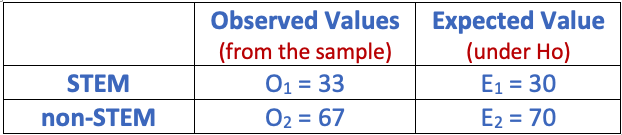
\includegraphics[width=0.5\linewidth]{week13/example01-ExpObsTable} \end{center}

In fact, a test statistic that measures the ``distance'' between the
observed and expected frequency tables and has a \(\chi^2\) (chi-square)
distribution is defined below \[
TS = \frac{(O_1 - E_1)^2}{E_1} + \frac{(O_2 - E_2)^2}{E_2} \to \chi_1^2.
\]

The value of the test statistic in this example

\[TS = \frac{(33-30)^2}{30} + \frac{(67-70)^2}{70} = 9/30 + 49/70 = 3/10 + 7/10 = 1\]

With the above value of test statistic, we can make a statistical
decision on \(H_0\) based on a given significance level.

\hypertarget{chi-squares-distribution}{%
\subsection{Chi-squares Distribution}\label{chi-squares-distribution}}

The chi-square distribution is used to characterize the positive random
variable. Unlike normal and t distributions that have symmetric density
curves, the chi-square distributions (dependent on the degrees of
freedom) have skewed density curves.

\begin{center}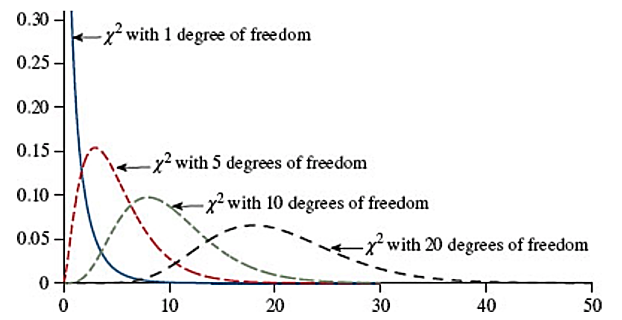
\includegraphics[width=0.6\linewidth]{week13/chisqDensity} \end{center}

We can find the critical value of chi-square distribution from the
chi-square table that is available on the course web page. The structure
of the chi-square table is similar to the t-table.

\begin{center}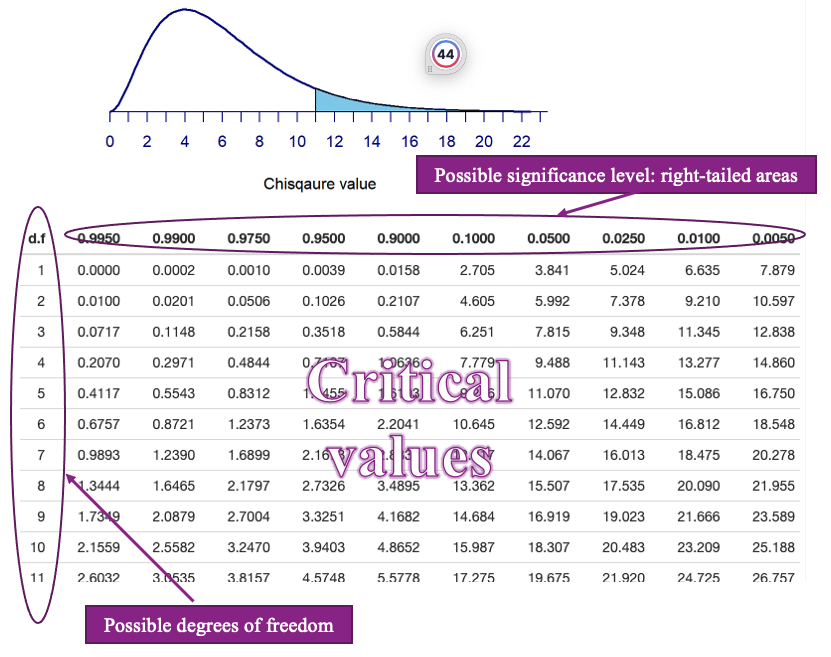
\includegraphics[width=0.8\linewidth]{week13/chisqTable} \end{center}

The possible degrees of freedom are listed in the first column, the
possible right-tail areas are listed in the top row, and the critical
values are listed in the main body of the table.

The steps for finding the critical values are the same as those we
followed for finding t- critical values.

\textbf{Example 2}. Find the critical value of the chi-square
distribution with 5 degrees of freedom with significance level 0.05.

\begin{center}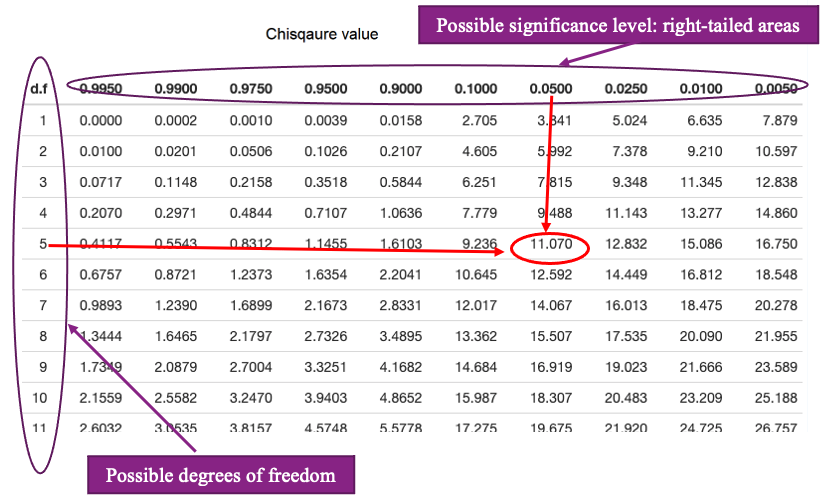
\includegraphics[width=0.8\linewidth]{week13/example02ChisqCV} \end{center}

The above figure shows how to find the critical value, denoted by
\(CV = \chi^2_{5, 0.05} = 11.071\). The first subscript denotes 5
degrees of freedom and the second subscript is the significance level of
0.05.

\hypertarget{formulation-of-chi-square-test-of-goodness-of-fit}{%
\subsection{Formulation of Chi-square Test of
Goodness-of-fit}\label{formulation-of-chi-square-test-of-goodness-of-fit}}

Let \(k\) be the number of categories of categorical variable \(Y\). The
category labels are \(C_1, C_2, \cdots, C_k\). Let
\(P_1 = Pr(C_1), P_2 = Pr(C_2), \cdots, P_k = Pr(C_k)\). The null
hypothesis claims that the categorical follows a specific distribution,
and the alternative hypothesis claims that the categorical distribution
does NOT follow the distribution specified in the null hypothesis. That
is, \[
H_0:\ \ P_1 = p_1, P_2 = p_2, \cdots, P_k = p_k \ \ \ \ v.s. \  \  \  \  H_a: \ \ the \ distribution \ in \ H_0 \ is \ not \ correct.
\] The \(N\) is the sample size. We can then calculate the
\textbf{expected cell frequency} of each category using formulas:
\(E_1 = N\times p_1, E_2 = N \times p_2, \cdots, E_k = N \times p_k\).
The \textbf{observed cell frequency}, denoted by \(O_i\) (for
\(i=1,2, \cdots, k\)), of each category is obtained from the data set.
The \textbf{expected} and \textbf{observed} frequencies are summarized
in the following table.

\begin{center}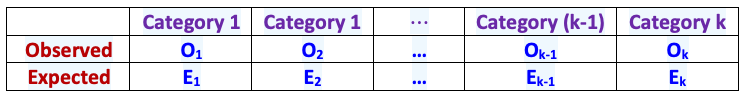
\includegraphics[width=0.6\linewidth]{week13/obsExpTable} \end{center}

The chi-square statistic is

\[
G^2 = \frac{(O_1-E_1)^2}{E_1} + \frac{(O_2-E_2)^2}{E_2} + \cdots + \frac{(O_k-E_k)^2}{E_k} \to \chi_{k-1}^2
\]

A small \(G^2\) indicates a lack of evidence for rejecting the null
hypothesis. This implies that \textbf{the Pearson chi-square test of
goodness is always a right-tailed test}. The degrees of freedom are
always \((k-1)\) if the categorical factor variable has k levels.

\textbf{Example 3}. A gambler wants to test a die to determine whether
it is fair. The gambler rolls a die that has six possible outcomes: 1,
2, 3, 4, 5, and 6; and the die is fair if each of these outcomes is
equally likely. The gambler rolls the die 60 times and counts the number
of times each number comes up. These counts, which are called the
observed frequencies, are

\begin{center}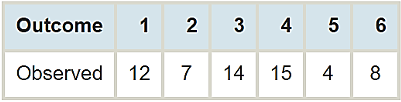
\includegraphics[width=0.35\linewidth]{week13/example03Data} \end{center}

\textbf{Solution}: The null hypothesis is that the six-sided die is
fair. That is equivalent to \[
H_0: \ \  p_1 = p_2 = p_3 = p_4 = p_5 = p_6 = 1/6 \ \ \ \ v.s. \ \ \ \ H_a: \ \ The \ die \ is \ NOT \ fair.
\] Based on the observed frequency table, the size of the sample is 60.
Using the \emph{cell probabilities} in \(H_0\), we have \textbf{expected
frequencies} of the 6 categories to be equal to 10. We summarize the
\textbf{expected} and \textbf{observed} frequencies in the following
table.

\begin{center}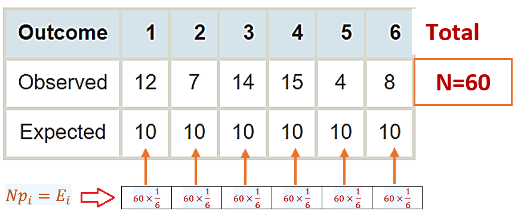
\includegraphics[width=0.45\linewidth]{week13/example03} \end{center}

The test statistic for testing \(H_0\) is defined by \[
G^2 = \frac{(12-10)^2}{10}+\frac{(7-10)^2}{10}+\frac{(14-10)^2}{10}+\frac{(15-10)^2}{10}
+\frac{(4-10)^2}{10}+\frac{(8-10)^2}{10} \\ =(4+9+16+25+36+4)/10=9.4
\] Since the categorical variable (number of dots on the faces of the
6-sided die) has 6 categories. The test statistic has 5 degrees of
freedom. The critical value based on the significance level of 0.05 is
given in the following figure

\begin{center}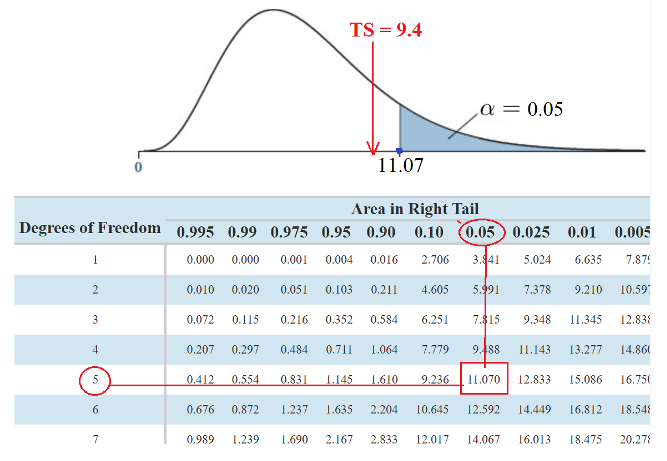
\includegraphics[width=0.85\linewidth]{week13/example03CV} \end{center}

The test statistic is NOT in the rejection region. We fail to reject the
null hypothesis. The die is a fair die.

\textbf{Example 4}. Grade distribution: A statistics teacher claims
that, on average, \(20\%\) of her students get a grade of A, \(35\%\)
get a B, \(25\%\) get a C, \(10\%\) get a D, and \(10\%\) get an F. The
grades of a random sample of 100 students were recorded. The following
table presents the sample frequencies of each grade.

\begin{center}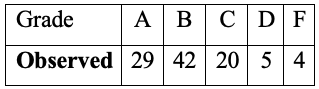
\includegraphics[width=0.25\linewidth]{week13/example04Data} \end{center}

\textbf{Solution}: Based on the given information. \(N = 100\). The null
hypothesis and the alternative hypothesis are \[
H_0: \ \ p_A = 0.2, p_B = 0.35, p_C = 0.25, p_D = 0.1, p_F = 0.1 \ \ \ \ v.s. H_a: \ \ The \ claimed \ distribution \ is \ wrong.
\] Under the null hypothesis, the expected table is given by

\begin{center}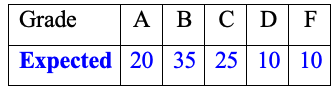
\includegraphics[width=0.25\linewidth]{week13/example04ExpTable} \end{center}

The test statistic has 4 degrees of freedom and the value is calculated
as follows \[
G^2=\frac{(29-20)^2}{20}+\frac{(42-35)^2}{35}+\frac{(20-25)^2}{25}+\frac{(5-10)^2}{10}+\frac{(4-10)^2}{10}=12.56
\] The critical value with a significance level of 0.05 is given by

\begin{center}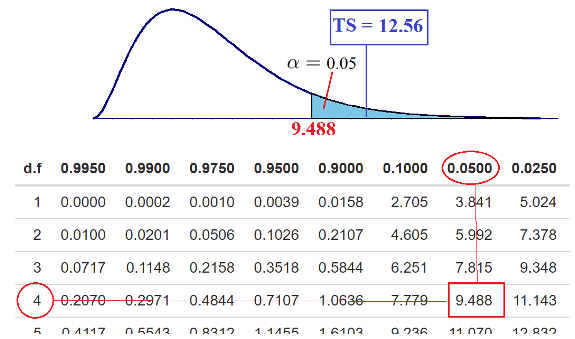
\includegraphics[width=0.75\linewidth]{week13/example04CV} \end{center}

Since the test statistic is inside the rejection region, we reject the
null hypothesis. That is, the sample does not support the claimed grade
distribution in \(H_0\).

\textbf{Remark}: In the chi-square goodness-of-fit test, the crucial
step is to find the *expected** frequency table under the null
hypothesis.

\hfill\break

\textbf{Here is another example that is different from the above
example}

\hfill\break

\hfill\break

\hypertarget{chi-square-test-of-independence}{%
\section{Chi-square Test of
Independence}\label{chi-square-test-of-independence}}

Let \(X\) and \(Y\) be two categorical variables with \(k\) and \(m\)
categories respectively. Their relationship between \(X\) and \(Y\) is
characterized by their joint distribution (table). For simplicity, we
use the following two special categorical to explain the ideas of
statistical testing of independence.

\hypertarget{independence-of-two-categorical-variables}{%
\subsection{Independence of Two Categorical
Variables}\label{independence-of-two-categorical-variables}}

We use the following example to illustrate \textbf{independence} and
\textbf{dependence} between two categorical variables.

\textbf{Example 5}. \emph{Joint probabilities and contingency tables.}
Let \(X =\) political preference (Democrat vs Republican) and
\(Y =\)gender (Male and Female). Let's \textbf{assume} their joint
distribution to be of the following \emph{contingency table}.

\begin{center}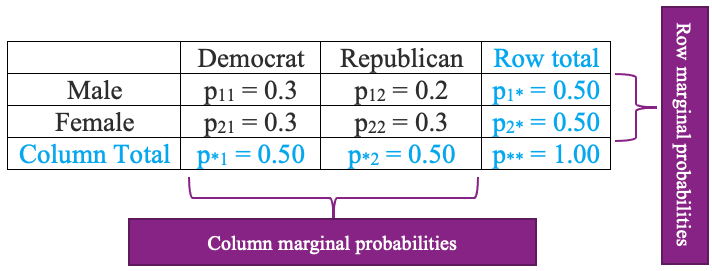
\includegraphics[width=0.65\linewidth]{week13/twoWayContingencyTable} \end{center}

The cell numbers are joint probabilities. For example,
\(p_{12} = 0.2 = 20\%\) says \(20\%\) of the \emph{study population} are
male republicans. The row and column totals represent the percentage of
male/female and democrats/republicans in the study population. Any
observed data table is \textbf{governed} by the above joint distribution
table.

\textbf{Definition} Two categorical variables are \textbf{independent}
if and only if their joint probabilities are equal to the product of
their corresponding marginal probabilities.

With this definition, we can see that \(X\) and \(Y\) with joint
distribution specified in the above table (in Example 5) ar NOT
independent since \(p_{11} =0.3 \ne 0.5\times 0.5 = 0.25\).

\textbf{Example 6}. We consider two variables \(X =\) preference of hair
color (Blonde and Brunette) and \(Y =\) gender (Male and Female). Assume
the joint distribution of the two variables is given by

\begin{center}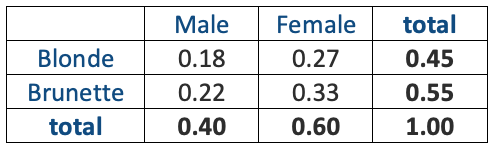
\includegraphics[width=0.35\linewidth]{week13/independenceContingencyTable} \end{center}

Based on the definition of independence. The preference for hair color
is independent of gender. Since \textbf{all} joint probabilities are
equal to the product of their corresponding marginal probabilities.

\(0.45\times 0.40 = 0.18, 0.45 \times 0.60 = 0.27, 0.55 \times 0.40 = 0.22\),
and \(0.55 \times 0.60 = 0.33.\)

\hypertarget{expected-table-under-independence-assumption-h_0}{%
\subsection{\texorpdfstring{Expected Table Under Independence Assumption
(\textbf{\(H_0\)})}{Expected Table Under Independence Assumption (H\_0)}}\label{expected-table-under-independence-assumption-h_0}}

We construct the \textbf{expected table} under the \textbf{null
hypothesis of independence} and the \textbf{observed contingency table}.
For ease of interpretation, we use an example to illustrate the steps
for obtaining the expected table.

\textbf{Example 7}. Consider the potential dependence between the
attendance (good vs poor) and course grade (pass vs fail). We take 50
students from a population and obtain the following observed table.

\begin{center}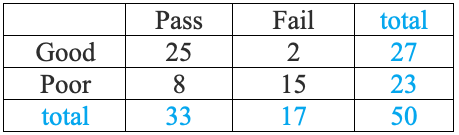
\includegraphics[width=0.35\linewidth]{week13/attendancePassFail} \end{center}

\textbf{Question}: Whether the attendance is independent of class
performance? \[
Ho: \ \ attendance \ is \ \ independent \ \ of \ the \ performance
\] \[versus\]

\[
Ha: \ \ attendance \ is  \ \ dependent \ of \ the \ performance
\]

To obtain the expected table, we follow the next few steps.

\begin{enumerate}
\def\labelenumi{\arabic{enumi}.}
\tightlist
\item
  Estimate the marginal probabilities
\end{enumerate}

\begin{center}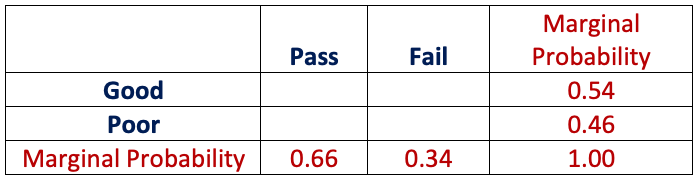
\includegraphics[width=0.5\linewidth]{week13/marginalTable} \end{center}

~~~~~~~~~~~where marginal probabilities are calculated by Pr(Good) =
27/50 = 0.54, Pr(Poor) = 23/50 = 0.46, Pr(Pass) = 33/50 = 0.66, Pr(Fail)
= 17/50 = 0.34.

\begin{enumerate}
\def\labelenumi{\arabic{enumi}.}
\setcounter{enumi}{1}
\tightlist
\item
  Estimate the joint probability under the null hypothesis of
  independence
\end{enumerate}

\begin{center}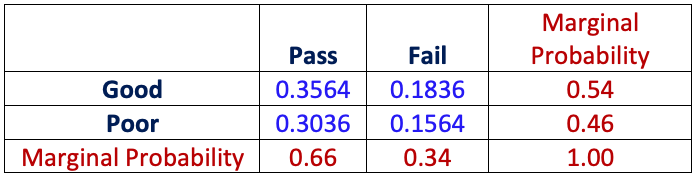
\includegraphics[width=0.5\linewidth]{week13/jointProb} \end{center}

~~~~~~~~~~~where joint probabilities under the independence assumption
(\(H_0\)) are calculated by taking the product of the corresponding
marginal probabilities. For example, 0.54 \(\times\) 0.66 = 0.3564.

\begin{enumerate}
\def\labelenumi{\arabic{enumi}.}
\setcounter{enumi}{2}
\tightlist
\item
  Calculate Expected Table
\end{enumerate}

~~~~~~~~~~The expected frequencies are calculated in the following table
(with detailed steps).

\begin{center}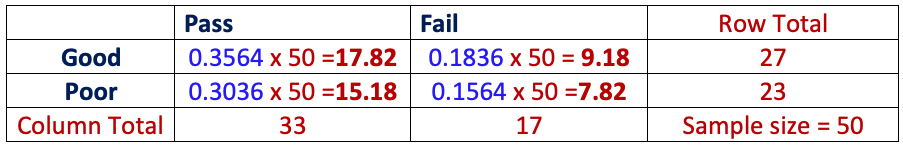
\includegraphics[width=0.65\linewidth]{week13/expectedTable} \end{center}

\hfill\break

\textbf{Remark}. For categorical variables with \textbf{more than two
categories}, the expected table can be found using ** the same 3 steps**
as those used in the above example.

\hfill\break

\hypertarget{formulation-of-chi-squares-test-of-independence}{%
\subsection{Formulation of Chi-squares Test of
Independence}\label{formulation-of-chi-squares-test-of-independence}}

The test statistic used to test the independence of two categorical
variables is the same as that used in the goodness-of-fit test. That is
the standardized ``distance'' between the observed and the expected
table (under \(H_0\)).

\textbf{Assume that the two categorical variables have \(k\) and \(m\)
categories respectively, then the resulting test statistic has a
chi-square distribution with \((k-1)\times(m-1)\) degrees of freedom.}

\textbf{Example 8}. {[}Continuation of \textbf{Example 7}{]}. Test
whether \textbf{attendance} and \textbf{class performance}.

\textbf{Solution}: We have found the expected table under \(H_0\) in
\textbf{Example 7}, we put the observed and expected tables in the
following.

\begin{center}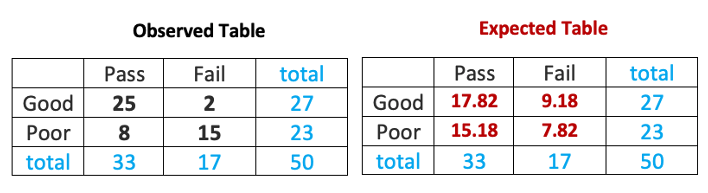
\includegraphics[width=0.7\linewidth]{week13/example08ExpObs} \end{center}

The test statistic is given by

\[
TS = \frac{(25-18.82)^2}{17.82} + \frac{(2-9.18)^2}{9.18} + \frac{(8-15.18)^2}{15.18} + \frac{(15-7.82)^2}{7.82} = 17.75
\]

The test statistic has a chi-square distribution with
\((2-1)\times (2-1) = 1\) degrees of freedom. The critical value at the
significance level of 0.05 is found in the following figure.

\begin{center}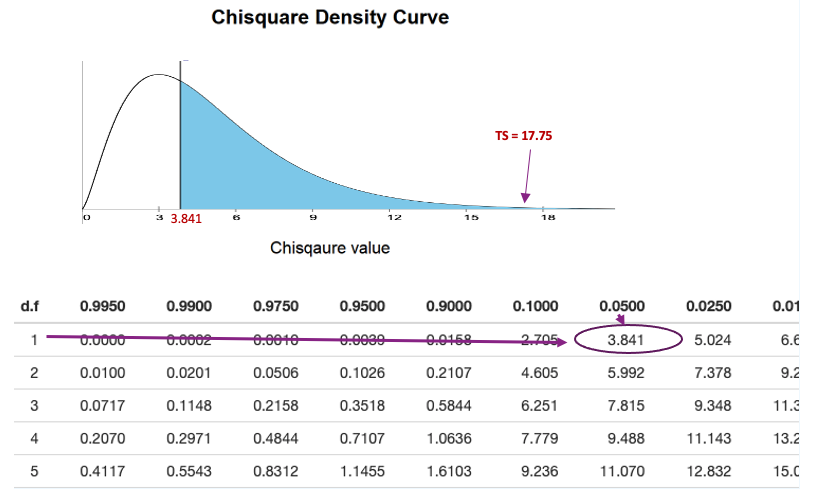
\includegraphics[width=0.85\linewidth]{week13/example08ChisqCV} \end{center}

Since the test statistic is inside the rejection region, we reject the
null hypothesis that attendance and class performance are independent.

\textbf{Example 9}. Do some college majors require more studying than
others? The National Survey of Student Engagement asked a number of
college freshmen what their major was and how many hours per week they
spent studying, on average. A sample of 1000 of these students was
chosen, and the numbers of students in each category are tabulated in
the following two-way contingency table.

\begin{center}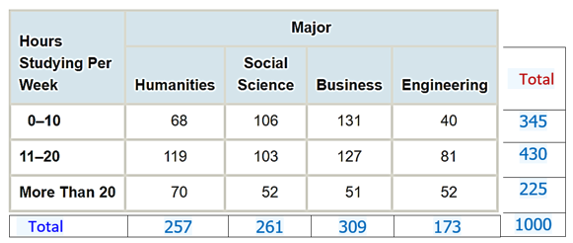
\includegraphics[width=0.6\linewidth]{week13/example09Data} \end{center}

\textbf{Solution}: The null and alternative hypotheses are given by

\begin{verbatim}
       Ho: studying time is INDEPENDENT on majors
                   versus
       Ha: studying time is DEPENDENT on majors.
\end{verbatim}

Under the null hypothesis, we obtained the expected table using the same
steps in Example 7 in the following.

\begin{center}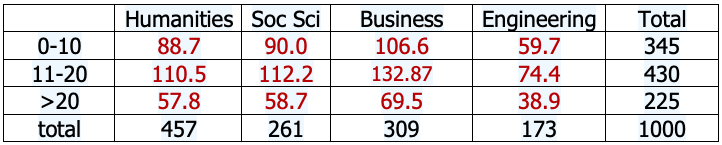
\includegraphics[width=0.55\linewidth]{week13/example09ExpTable} \end{center}

The test statistic is given by

\begin{center}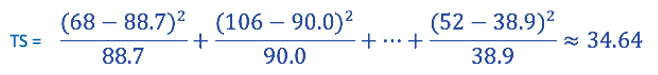
\includegraphics[width=0.6\linewidth]{week13/example09TS} \end{center}

The critical value and rejection region based on significance level 0.05
is given by

\begin{center}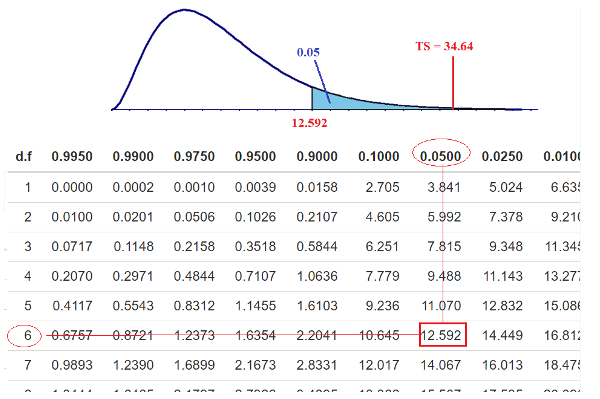
\includegraphics[width=0.8\linewidth]{week13/example09CV} \end{center}

\textbf{Conclusion}: Since the test statistic is inside the rejection
region, we reject the null hypothesis and conclude that the studying
time is dependent on the majors.

\hypertarget{use-of-technology}{%
\section{Use of Technology}\label{use-of-technology}}

Two apps were created for the two chi-square tests of goodness-of-fit
and independence respectively.

\hypertarget{goodness-of-fit-chi-square}{%
\subsection{Goodness-of-fit
Chi-square}\label{goodness-of-fit-chi-square}}

The app is at: \url{https://chpeng.shinyapps.io/chisq-gof/}. The
following screenshot illustrates the use of this app using Example 03 in
this note.

\begin{center}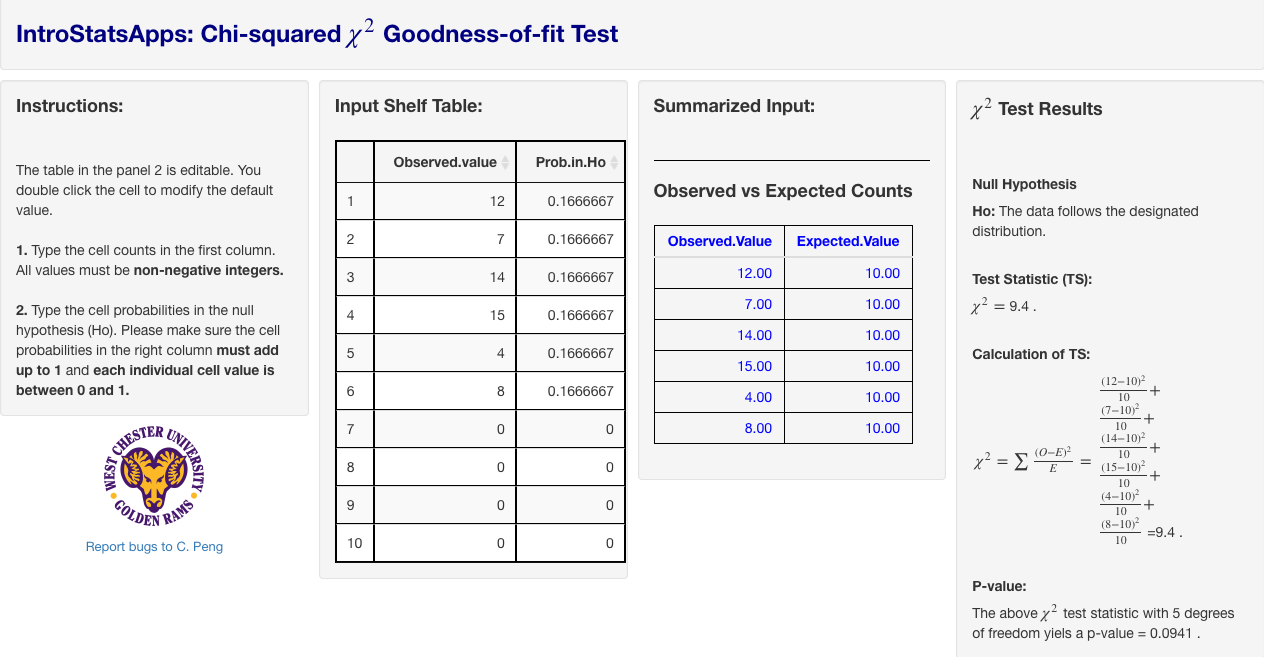
\includegraphics[width=1\linewidth]{week13/useTech01} \end{center}

\hypertarget{chi-square-test-of-independence-1}{%
\subsection{Chi-square Test of
Independence}\label{chi-square-test-of-independence-1}}

The app is at \url{https://chpeng.shinyapps.io/chisq-independence/}. We
use this app with Example 09.

\begin{center}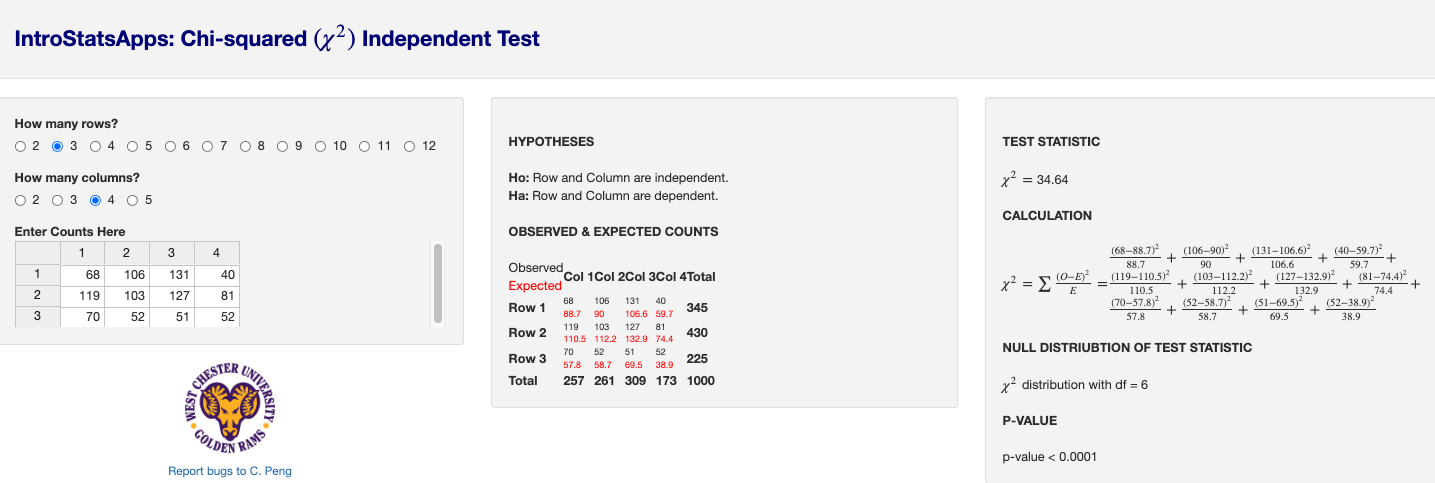
\includegraphics[width=1\linewidth]{week13/useTech02} \end{center}

\hfill\break

\hypertarget{practice-exercises}{%
\section{Practice Exercises}\label{practice-exercises}}

\hfill\break
\hfill\break
You can use the apps to do the following exercises.

\begin{enumerate}
\def\labelenumi{\arabic{enumi}.}
\tightlist
\item
  \textbf{College Sports}
\end{enumerate}

A University conducted a survey of its recent graduates to collect
demographic and health information for future planning purposes as well
as to assess students' satisfaction with their undergraduate
experiences. The survey revealed that a substantial proportion of
students were not engaging in regular exercise, many felt their
nutrition was poor and a substantial number were smoking. In response to
a question on regular exercise, 60\% of all graduates reported getting
no regular exercise, 25\% reported exercising sporadically and 15\%
reported exercising regularly as undergraduates. The next year the
University launched a health promotion campaign on campus in an attempt
to increase health behaviors among undergraduates. The program included
modules on exercise, nutrition, and smoking cessation. To evaluate the
impact of the program, the University again surveyed graduates and asked
the same questions. The survey was completed by 470 graduates and the
following data were collected on the exercise question:

\begin{center}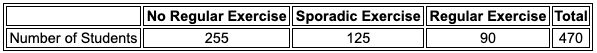
\includegraphics[width=0.75\linewidth]{week13/practiceEx01Data} \end{center}

We specifically want to compare the distribution of responses in the
sample to the distribution reported the previous year (i.e., 60\%, 25\%,
15\% reporting no, sporadic and regular exercise, respectively). Whether
the data supports the above distribution at a significance level of
0.05.

\begin{enumerate}
\def\labelenumi{\arabic{enumi}.}
\setcounter{enumi}{1}
\tightlist
\item
  \textbf{Political Affiliation and Opinion}
\end{enumerate}

The following table based on the sample will be used to explore the
relationship between Party Affiliation and Opinion on Tax Reform.

\begin{center}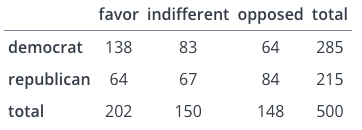
\includegraphics[width=0.35\linewidth]{week13/practiceEx02Data} \end{center}

Find the expected counts for all of the cells.

\begin{enumerate}
\def\labelenumi{\arabic{enumi}.}
\setcounter{enumi}{2}
\tightlist
\item
  \textbf{Tire Quality}
\end{enumerate}

The operations manager of a company that manufactures tires wants to
determine whether there are any differences in the quality of work among
the three daily shifts. She randomly selects 496 tires and carefully
inspects them. Each tire is either classified as perfect, satisfactory,
or defective, and the shift that produced it is also recorded. The two
categorical variables of interest are the shift and condition of the
tire produced. The data can be summarized by the accompanying two-way
table. Does the data provide sufficient evidence at the 5\% significance
level to infer that there are differences in quality among the three
shifts?

\begin{center}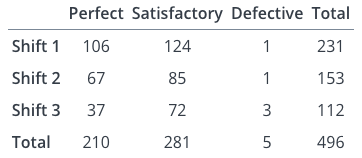
\includegraphics[width=0.35\linewidth]{week13/practiceEx03Data} \end{center}

\begin{enumerate}
\def\labelenumi{\arabic{enumi}.}
\setcounter{enumi}{3}
\tightlist
\item
  \textbf{Condiment preference and gender}
\end{enumerate}

A food services manager for a baseball park wants to know if there is a
relationship between gender (male or female) and the preferred condiment
on a hot dog. The following table summarizes the results. Test the
hypothesis with a significance level of 10\%.

\begin{center}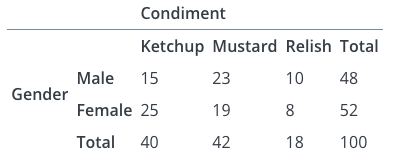
\includegraphics[width=0.35\linewidth]{week13/practiceEx04Data} \end{center}

\end{document}
